\chapter{Simulations}\label{Chapter:Simulations}

The model used to test all of the aforementioned theory is a simple, closed loop model with 14 control volume and 14 momentum cells.
The model's steady-states and stability were characterized and test both in single and two phase states.
The single phase tests were performed in the sub-cooled liquid regime of water over a chosen rectangle in pressure-temperature space at two different heating loads.
The two-phase tests were performed along the saturated liquid line of the vapor dome over several saturation temperatures at four different heating loads.

\section{Solution Methology}

Despite the simple geometry, the steady-state solutions required for the stability analysis are not easily solved because any closed-loop system presents an inherently singular steady-state balance between fluxes and sources.
Therefore, all of the steady-states that will be presented were acquired from transient simulations that were run until the absolute value of the time rate-of-change of all system variables fell below 10.
The limiting variable using that metric was the energy of the control volumes since their values were on the order of \SIrange{1E5}{1E6}{\joule} with all other system variables being driven to very small rates-of-change relative to their inherent scales.

The eigenvalue calculations were performed using a central finite difference on the momentum value to approximate the required derivatives.
A numerical approximation was chosen to overcome the complexities of the derivatives due to models used in single phase and primarily those in two-phase for the friction factor multiplier.


\begin{figure}[t]%
    \centering
    \caption{Test loop geometry.  Black lines enclose control volumes, dashed red lines indicate the extents of the momentum cells, the blue control volume is removing the heat load, and the yellow control volume is receiving the heat load.}%
    \label{Fig:TestLoopSetUp}%
    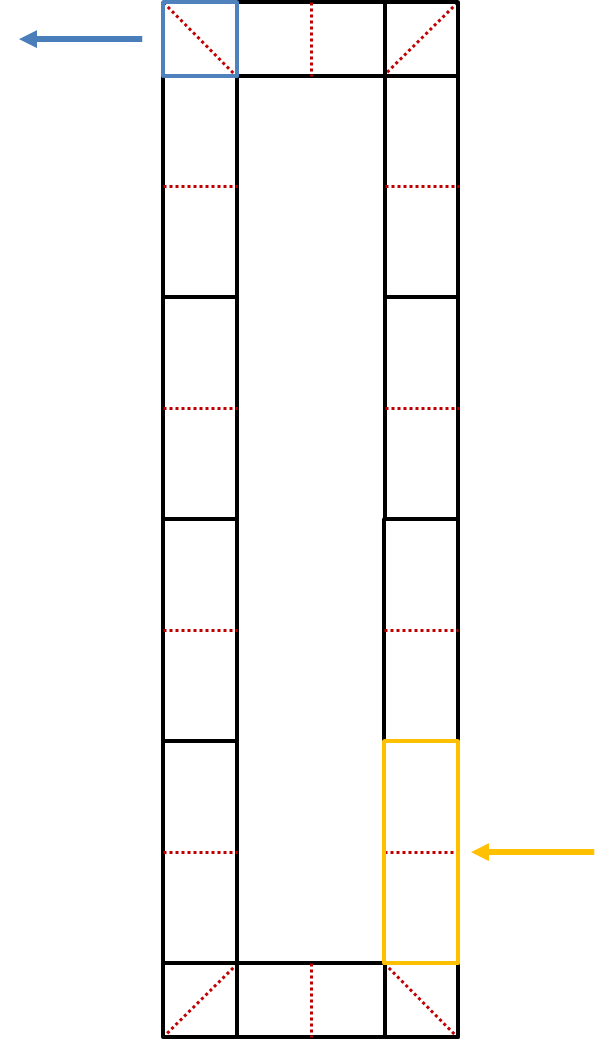
\includegraphics[height=4in]{TestLoop.png}%
\end{figure}


\section{Geometry}

The loop geometry and problem set-up are summarized in \cref{Fig:TestLoopSetUp}.
All of the control volumes have a hydraulic diameter or \SI{0.1}{\meter} and exchange surface flow areas of \SI{1E-2}{\meter\squared}.
The lengths of the corner volumes is \SI{0.1}{\meter} on all sides, the horizontal bridges are \SI{0.2}{\meter} in length, and the vertical volumes are \SI{0.3}{\meter} tall.
The total volume of the system is \SI{0.032}{\meter\cubed} with an aspect ratio of \num{3.5}.

The geometry was chosen to be a smaller scale version of the UW--Madison RCCS experiment.
The size of the model, number of control volumes, and total amount of water in the system has an enormous impact on the current performance of the code used to solve the problems.
As such, a small numerical experiment was settled upon to allow efficient investigation into both the single and two-phase systems before any in-depth efforts were made to improve performance beyond the code optimizations of the implementation language and platform.


\begin{table}[b]%
    \centering
    \centering
    \caption{Summary of pertinent system parameters for the single phase simulations.}
    \label{Table:1PhiSummary}
    \begin{tabular}{ccc}
        \toprule
            \multirow{2}{*}{Parameters} & \multicolumn{2}{c}{Heat Load} \\[0.1em]\cline{2-3}
                                       &    \SI{1}{\kW} & \SI{8}{\kW} \\\midrule
        Avg. Temperature Rise    [\si{\Delta\kelvin}] & \num{0.2392}   & \num{0.7944} \\[0.5em]
        Avg. Pressure Difference [\si{\Delta\kilo\pascal}]  & \num{12.504} & \num{12.500} \\[0.5em]
        Avg. Mass Flow Rate      [\si{\kg\per\second}]      & \num{1.012}    & \num{2.437} \\[0.5em]
        $\dot{m}c\subs{p}\Delta{T}$ [\si{\kW}]*            & \num{1.02}     & \num{8.097}\\
        \bottomrule
    \end{tabular}
    \vskip0pt
    * $c\subs{p} = \SI{4182}{\joule\per\kg\per\kelvin}$
\end{table}

\section{Single Phase Results}

The single phase simulations were carried out by setting the cooling corner of the model to a set temperature and pressure and letting the simulation run to a steady-state.
Steady-states were generated using a grid of temperatures ranging from \SIrange{300}{372}{\kelvin} and pressure ranging from \SIrange{101325}{202650}{\pascal} and heat loads of \SI{1}{\kW} and \SI{8}{\kW}.
Pertinent average parameters and a crude energy balance for comparison are presented in \cref{Table:1PhiSummary}.


The results of the eigenvalue calculations over the computational rectangles are presented in \cref{Fig:Eigenvalue1kW,Fig:Eigenvalue8kW}.
As can be seen, all of the computed eigenvalues are below zero, and thus the system doesn't exhibit any instabilities in the single phase region.
The lack of a boundary is not all that shocking given that water is an extremely dense and robust fluid while it is in the subcooled regime.
Additionally, since the only remaining system-wide terms in the perturbation equations were dissipative in nature, the absolute stability of the simulations is not that surprising.
It is noted, however, that the eigenvalues for the \SI{8}{\kW} heat load are an order of magnitude higher than the \SI{1}{\kW} simulation, and future simulations examining behavior at higher heating levels is worth considering.


\section{Two-Phase Results}

The two-phase simulations were carried out by setting the cooling corner of the model to a saturation temperature with the associated pressure and liquid density; the system was then heated and allowed to evolve to a steady-state.
Steady-states were generated using saturation temperatures ranging from \SIrange{372}{390}{\kelvin}, which corresponds to a pressure range of \SIrange{97.33}{179.64}{\kilo\pascal}, with heat loads of \num{1}, \num{2}, \num{4}, and \SI{6}{\kW}.
Pertinent average parameters and a crude energy balance for comparison are presented in \cref{Table:2PhiSummary}.

\begin{table} 
    \centering
    \centering
    \caption{Summary of pertinent system parameters for the two-phase simulations.}
    \label{Table:2PhiSummary}
    \begin{tabular}{ccccc}
        \toprule
            \multirow{2}{*}{Parameters}                     & \multicolumn{4}{c}{Heat Load} \\[0.1em]\cline{2-5}
                                                            &    \SI{1}{\kW} & \SI{2}{\kW}   & \SI{4}{\kW}   & \SI{6}{\kW} \\\midrule
        Avg. Temperature Rise    [\si{\Delta\kelvin}]       & \num{0.034}    & \num{0.0352}  & \num{0.0951}  & \num{0.13}  \\[0.5em]
        Avg. Pressure Difference [\si{\Delta\kilo\pascal}]  & \num{12.17}    & \num{12.17}   & \num{12.29}   & \num{12.38} \\[0.5em]
        Avg. Mass Flow Rate      [\si{\kg\per\second}]      & \num{6.89}     & \num{6.97}    & \num{9.92}    & \num{10.89} \\[0.5em]
        Avg. Maximum Quality      [--]                      & \num{6.48E-5}  & \num{6.71E-5} & \num{1.68E-4} & \num{2.22E-4} \\[0.5em]
        \bottomrule
    \end{tabular}
\end{table}


The results of the eigenvalue calculations over the saturation temperatures and across the powers is presented in \cref{Fig:2PhiEigenvalues}.
As can be seen, all of the computed eigenvalues are below zero, and thus the system doesn't exhibit any instabilities when portions of the upper hot leg undergo flashing.
The lack of a any positive eigenvalues is a little surprising given the chaotic nature two-phase flash is known to have.
However, the state space presented is not that refined, so there may be positions along the saturation line that were not captured in these simulations.
Additionally, the heating levels turned out to be two low for even a modestly wet two-phase mixture, not even achieving a tenth of a percent in quality.
Refinement of the simulation state space and higher power levels are left to future work.


\begin{figure}%
    \caption{Eigenvalue map of the simple, closed loop over the chosen state space. All eigenvalues are negative}%
    \begin{subfigure}{\textwidth}
        \centering
        \caption{\SI{1}{\kW}}
        \label{Fig:Eigenvalue1kW}
        \vskip-1.1em
        \IncludeSection{EigenvalueMap_SinglePhase_1kW.tikz}%
    \end{subfigure}
    \vskip1.5em
    \begin{subfigure}{\textwidth}
        \centering
        \caption{\SI{8}{\kW}}
        \label{Fig:Eigenvalue8kW}
        \vskip-0.75em
        \IncludeSection{EigenvalueMap_SinglePhase_8kW.tikz}%
    \end{subfigure}
\end{figure}

\begin{figure}%
    \centering
    \caption{Eigenvalue map of the simple, closed loop undergoing phase-change along the liquid saturation line at various heating loads.All eigenvalues are negative}%
    \label{Fig:2PhiEigenvalues}
    \vskip-0.75em
    \IncludeSection{EigenvalueMap_TwoPhase_1kW.tikz}%
\end{figure}
